\documentclass{book}
\providecommand{\draftversion}{no}
%----------------------------------------------------------------------------
\usepackage{fancybox}
\usepackage{fancyvrb}
\usepackage{syntax}
\usepackage{url}
\usepackage{graphicx}
\usepackage{amsmath}
\usepackage{xspace}

%----------------------------------------------------------------------------
\usepackage[paper=a4paper]{geometry}
\usepackage{microtype}
\usepackage{cite}
\usepackage{makeidx}
\usepackage{watermark}
\usepackage{ifthen}
\usepackage{tikz}
\usepackage{environ}
\usepackage{listings}
\usetikzlibrary{fadings}
\usetikzlibrary{calc}
%----------------------------------------------------------------------------
%\usepackage{showidx}	%%% NOTE: Only for DRAFT!
%----------------------------------------------------------------------------
\makeindex 
%----------------------------------------------------------------------------

%----------------------------------------------------------------------------
\begin{document}
% Assist
\newcommand{\z}[1]{\mathit{#1}}                    %text in math mode, keep size using amstext

% For the MSC
\newcommand{\synch}{\z{ni\text{-}synch}}           %synchronization claim
\newcommand{\isynch}{\z{i\text{-}synch}}           %synchronization claim
\newcommand{\agree}{\z{ni\text{-}agree}}           %full agreement claim
\newcommand{\iagree}{\z{i\text{-}agree}}           %injective full agreement claim
\newcommand{\secret}{\z{secret}}           %secrecy claim
\newcommand{\enc}[2]{\{{#1}\}_{#2}}      %Encryption
\newcommand{\nI}{ni}
\newcommand{\nR}{nr}
\newcommand{\nS}{ns}
\newcommand{\nb}{nb}
\newcommand{\pkIinv}{sk(I)}
\newcommand{\pkRinv}{sk(R)}
\newcommand{\pkSinv}{sk(S)}
\newcommand{\pkbinv}{sk(b)}
\newcommand{\pkI}{pk(I)}
\newcommand{\pkR}{pk(R)}
\newcommand{\pkS}{pk(S)}

%%% Abbreviation macros
\newcommand{\ie}{i.\@\,e.\@\xspace}
\newcommand{\eg}{e.\@\,g.\@\xspace}
\newcommand{\wrt}{w.\@\,r.\@\,t.\@\xspace}
\newcommand{\st}{s.\@\,t.\@\xspace}
\newcommand{\etc}{etc.\@\xspace}
\newcommand{\etal}{et~al.\@\xspace}

\newcommand{\spdindex}[1]{\index{#1@\spd{#1}}}
%----------------------------------------------------------------------------
%
% NOTE TO FRIENDS: Please use the macro below to insert remarks at
% various points. Usage: \remark{A friend}{This is great!}
%
\ifthenelse{\equal{\draftversion}{yes}}
{
\newcommand{\remark}[2]{

{\bf Draft note (#1)} : {\em #2}

}
\newcommand{\later}{

{\em More text will be supplied at a later stage.}

}
}{
\newcommand{\remark}[2]{}
\newcommand{\later}{To be continued\ldots}
}

%----------------------------------------------------------------------------
%----------------------------------------------------------------------------

% Environments
\newenvironment{example}{}{}

\DefineVerbatimEnvironment
  {screen}{Verbatim}
  {fontsize=\small,frame=lines,fontfamily=courier}
\DefineVerbatimEnvironment
  {ingraph}{Verbatim}
  {frame=single,xleftmargin=1.0cm,xrightmargin=1.0cm}
\DefineVerbatimEnvironment
  {email}{Verbatim}
  {fontfamily=courier}
\DefineVerbatimEnvironment
  {spdlFV}{Verbatim}
  {frame=single,xleftmargin=1.0cm,xrightmargin=1.0cm}
\newcommand{\spd}[1]{{\tt #1}}
\newcommand{\scr}[1]{{\tt #1}}
\newcommand{\gra}[1]{{\tt #1}}



\lstnewenvironment{spdl}{%
  \lstset{backgroundcolor=\color{verbgray},
  frame=single,
  framerule=0.5pt,
  rulecolor=\color{verbgrayframe},
  basicstyle=\small\ttfamily,
  xleftmargin=10pt,
  xrightmargin=10pt,
  columns=fullflexible}}{}

%----------------------------------------------------------------------------

\pagestyle{headings}

%----------------------------------------------------------------------------
%
%	FRONT PAGE
%
\thispagestyle{empty}

\definecolor{verbgray}{HTML}{F0F0F0}		% Background of code listings
\definecolor{verbgrayframe}{HTML}{C0C0C0}	% Background of code listings' frames
\definecolor{lgrey}{HTML}{C0E0FF}		% Background of "new since" tabs
\definecolor{sblue}{HTML}{26546C}
\definecolor{lblue}{HTML}{E8F8FF}
\definecolor{gblue}{HTML}{6C6C6C}
\definecolor{sorange}{HTML}{E67400}
\definecolor{lorange}{HTML}{FFF8F0}
\definecolor{gorange}{HTML}{E6E6E6}
\definecolor{syellow}{HTML}{FBE115}

\begin{tikzpicture}[remember picture,overlay,
    titletext/.style={text=black,inner sep=0pt,anchor=south west,font=\sf,align=left}
  ]
  % Define coordinates
  \node (a) at (current page.north west) {};
  \node (b) at (current page.north east) {};
  \node (e) at (current page.south west) {};
  \node (f) at (current page.south east) {};
  \node (c) at ($ (e) + (0mm,200mm) $) {};
  \node (d) at ($ (f) + (0mm,200mm) $) {};
  \node (x) at ($ (c) + (0mm, 4pt) $) {};
  \node (y) at ($ (c) + (0mm,-4pt) $) {};
  % Orange upper
  %\fill[top color=white, bottom color=lorange]
  %  (a) rectangle ($ (d) + (0mm,-1mm) $);
  \fill[sorange]
    (x) rectangle ($ (d) + (0mm,-1mm) $);
  % Bottom blue
  %  \fill[top color=lblue, bottom color=white]
  %  (c) rectangle (f);
  % Blue center bar narrow
  \fill[sblue]
    (y) rectangle (d);
  % Yellow
  \fill [syellow]
    (y) rectangle ($ (y) + (8mm,-32mm) $);
  % Help grid
  %\draw[help lines,step=10mm] (e) grid (20,30);
  % Text
  \node[titletext,scale=10] 
    at ($ (e) + (30mm,145mm) $)
    {Scyther};
  \node[titletext,scale=6] 
    at ($ (e) + (30mm,125mm) $)
    {User Manual};
  \node[titletext,scale=3] 
    at ($ (e) + (60mm,235mm) $)
    {Cas Cremers};
    %{Cas Cremers\\Sjouke Mauw};  %% Until now, one man effort

  % Draft
  \node[titletext,scale=2,anchor=south] 
    at ($ (e) + (105mm,30mm) $)
    {Draft \today};
\end{tikzpicture}
%----------------------------------------------------------------------------
%
% Headers
%
\newcommand{\mygheaderA}{
  % Define coordinates
  \node (a) at ($ (current page.north west) + (0mm,-25mm) $) {};
  \node (b) at ($ (current page.north east) + (0mm,-25mm) $) {};
  \node (c) at ($ (a) + (0mm,-5mm) $) {};
  \node (d) at ($ (b) + (0mm,-5mm) $) {};
  \node (e) at ($ (c) + (0mm,-7mm) $) {};
  \node (f) at ($ (d) + (0mm,-7mm) $) {};
  % Orange upper
  \draw[draw=none] 
    [fill=gorange]
    (a) rectangle ($ (d) + (0mm,-1mm) $);
  \draw[draw=none] 
    [postaction={path fading=north,fill=sorange}]
    (a) rectangle ($ (d) + (0mm,-1mm) $);
  % Bottom blue
%  \draw[draw=none] 
%    [fill=gblue]
%    (c) rectangle (f);
  \draw[draw=none] 
    [postaction={path fading=south,fill=sblue}]
    (c) rectangle (f);
  % Yellow highlight
  \tikzfading[name=fade out,
    inner color=transparent!0,
    outer color=transparent!100]
}
\newcommand{\mygheaderB}{
  \draw[draw=none] 
    [postaction={path fading=north,fill=white}]
    (c) rectangle (f);
}
\newsavebox{\myheaderL}
\newsavebox{\myheaderR}
\savebox{\myheaderL}{
\begin{tikzpicture}[remember picture,overlay,
    titletext/.style={text=white,inner sep=0pt,anchor=south west,font=\sf,align=left}
  ]
  \mygheaderA
  \begin{scope}
    \draw[draw=none,clip]
      (c) rectangle (f);
    \fill [syellow,path fading=fade out]
      ($ (d) + -1.0*(30mm,90mm) $) rectangle ($ (d) + (30mm,90mm) $);
  \end{scope}
  \mygheaderB
\end{tikzpicture}
}
\savebox{\myheaderR}{
\begin{tikzpicture}[remember picture,overlay,
    titletext/.style={text=white,inner sep=0pt,anchor=south west,font=\sf,align=left}
  ]
  \mygheaderA
  \begin{scope}
    \draw[draw=none,clip]
      (c) rectangle (f);
    \fill [syellow,path fading=fade out]
      ($ (c) + -1.0*(30mm,90mm) $) rectangle ($ (c) + (30mm,90mm) $);
  \end{scope}
  \mygheaderB
\end{tikzpicture}
}
%\leftwatermark{\usebox{\myheaderL}}
%\rightwatermark{\usebox{\myheaderR}}


% NOTE for use of the 'supported' macro for denoting new features.
%
% \subsection[RealTitle]{RealTitle\supported{MyVersion and YourVersion}}
%
% The square-bracket version is needed, otherwise the 'new' bar shows up
% in the table of contents.
\newcommand{\supported}[1]{ 
	\hfill
	\colorbox{lgrey}{{\text{\small New in version #1}}
}}

%----------------------------------------------------------------------------
\tableofcontents
%----------------------------------------------------------------------------

%----------------------------------------------------------------------------
\chapter{Introduction}
%----------------------------------------------------------------------------

\begin{center}
\fbox{\parbox{0.8\textwidth}{
		\sf {\bf Note:} This is a draft of the new version of the Scyther manual. The manual may therefore be
incomplete at points.

Any feedback is
welcome and can be sent to Cas Cremers by e-mail:
{\tt cas.cremers@cs.ox.ac.uk}.
}}
\end{center}

\bigskip

\noindent
This is the user manual for the Scyther security protocol verification
tool.

The purpose of this manual is to explain the
details of the Scyther input language, explain how to model basic
protocols, and how to effectively use the Scyther tool.
This manual does not detail the protocol execution model nor
the adversary model used by the tool. It is therefore highly recommended to read the
accompanying book~\cite{opsembook}. The book includes a detailed
description of Scyther's
underlying protocol model, security property specifications, and the
algorithm.

We proceed in the following way. Some background is given in
Chapter~\ref{sec:background}. 
Chapter~\ref{sec:install} explains how to install the Scyther tool on
various platforms. In Chapter~\ref{sec:tutorial} we give a brief
tutorial using simple examples to show the basics of the tool.
Then we discuss things in more detail as we introduce the input language
of the tool in Chapter~\ref{sec:input}. Modeling of basic protocols is
described in Chapter~\ref{sec:modeling}, and
Chapter~\ref{sec:properties} describes how to specify security
properties. The usage of the GUI version of tool
is then explained in more detail in Section~\ref{sec:gui}. The
underlying command-line tool is described in Section~\ref{sec:cli}.
Advanced topics are discussed
in Section~\ref{sec:advanced}.

\section*{Online information}

More help can be found online on the Scyther website:

\index{Scyther website}
\index{website|see{Scyther website}}
\medskip
\url{http://users.ox.ac.uk/~coml0529/scyther/index.html}
\medskip

\noindent
Users are advised to subscribe to the Scyther mailing list,
whose details can also be found on the Scyther website.

%----------------------------------------------------------------------------
\chapter{Background}
\label{sec:background}
%----------------------------------------------------------------------------

Scyther is a tool for the formal analysis of security protocols under the
\emph{perfect cryptography assumption}, in which it is assumed that all
cryptographic functions are perfect: the adversary learns nothing from
an encrypted message unless he knows the decryption key. The tool can be
used to find problems that arise from the way the protocol is
constructed. This problem is undecidable in general, but in practice
many protocols can be either proven correct or attacks can be found.

The full protocol model, its assumptions, the basic security properties,
and the algorithm are described in~\cite{opsembook}. This manual serves
as a companion to the book.  Thus, in this manual we assume the
reader is familiar with the formal modeling of security protocols and
their properties.

% Not only is knowledge of security protocol models needed to use the
% Scyther tool, further knowledge is needed to know how to interpret the
% results that the tool produces in any useful way. In fact, the reader
% should be very cautious: security protocol models and their properties
% are intricate and it is easy to misinterpret the results.
% 
% Having said that, one of the main goals of Scyther is to help with the
% analysis of a protocol in such a way that for example attacks can be
% understood well. Thus, wherever possible the tool will give useful
% information on the results.

%----------------------------------------------------------------------------
\chapter{Installation}
\label{sec:install}
%----------------------------------------------------------------------------

Scyther can be downloaded from the following website:

\index{downloading Scyther}
\url{http://users.ox.ac.uk/~coml0529/scyther/}

\medskip

\noindent
\index{installing Scyther}
Installation instruction are included in the downloadable Scyther
archives. Scyther is available for the Windows,
Linux and Mac OS platforms.

%\section{Linux}

%\section{Windows}

%\section{MAC OS X}



%----------------------------------------------------------------------------
\chapter{Quick start tutorial}
\label{sec:tutorial}
%----------------------------------------------------------------------------

\index{quick start tutorial}
Scyther takes as input a security protocol description that includes a
specification of intended security properties, referred to as security
claims, and evaluates these. 

Start Scyther by executing the \scr{scyther-gui.py} program in the
Scyther directory. The program will launch two windows: the main window,
in which files are edited, and the \scr{about} window, which shows some
information about the tool. 

As an introductory example, we will verify the Needham-Schroeder
protocol, and investigate an attack on it. 

Go to the file$\rightarrow$open dialog, and open the file
\scr{ns3.spdl} in the Scyther directory. Your main window should look
like the one in Figure~\ref{protocolwindow}.

\begin{figure}[!htb]
  \begin{center}
    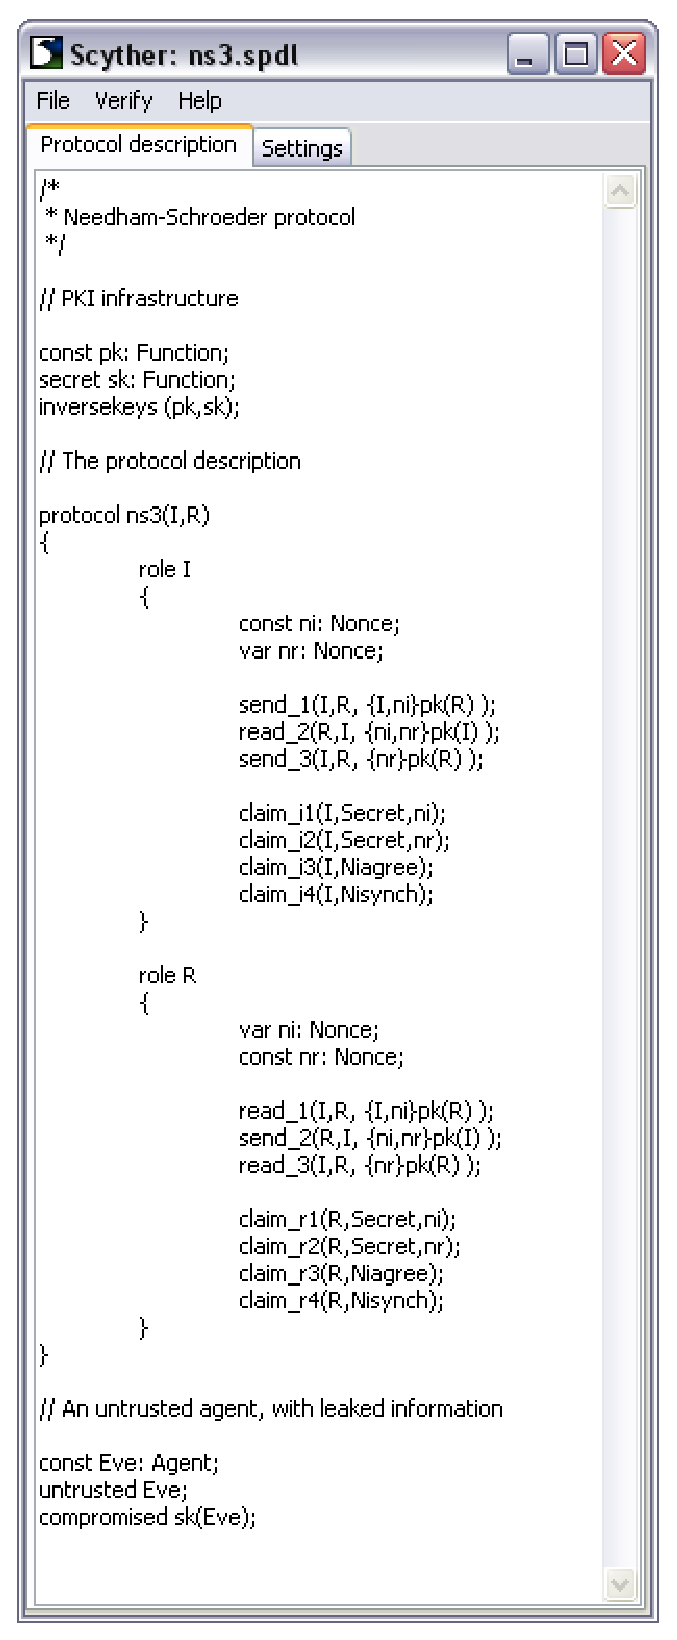
\includegraphics[height=0.90\textheight]{protocolwindow}
  \end{center}
  \label{protocolwindow}
  \caption{Scyther main window with the file ns3.spdl opened}
\end{figure}

By
convention, protocol description files have the extension \scr{.spdl} (Security Protocol Description
Language), but it can have any name. The file used in this example is
shown in Appendix~\ref{app:ns3}.

Run the verification tool by selecting verify$\rightarrow$verify\_claims in the
menu. A new window will appear during the verification process. Once
verification is completed, the window will be
replaced by the result window, as shown in
Figure~\ref{resultwindow}.

\begin{figure}[!htb]
  \begin{center}
    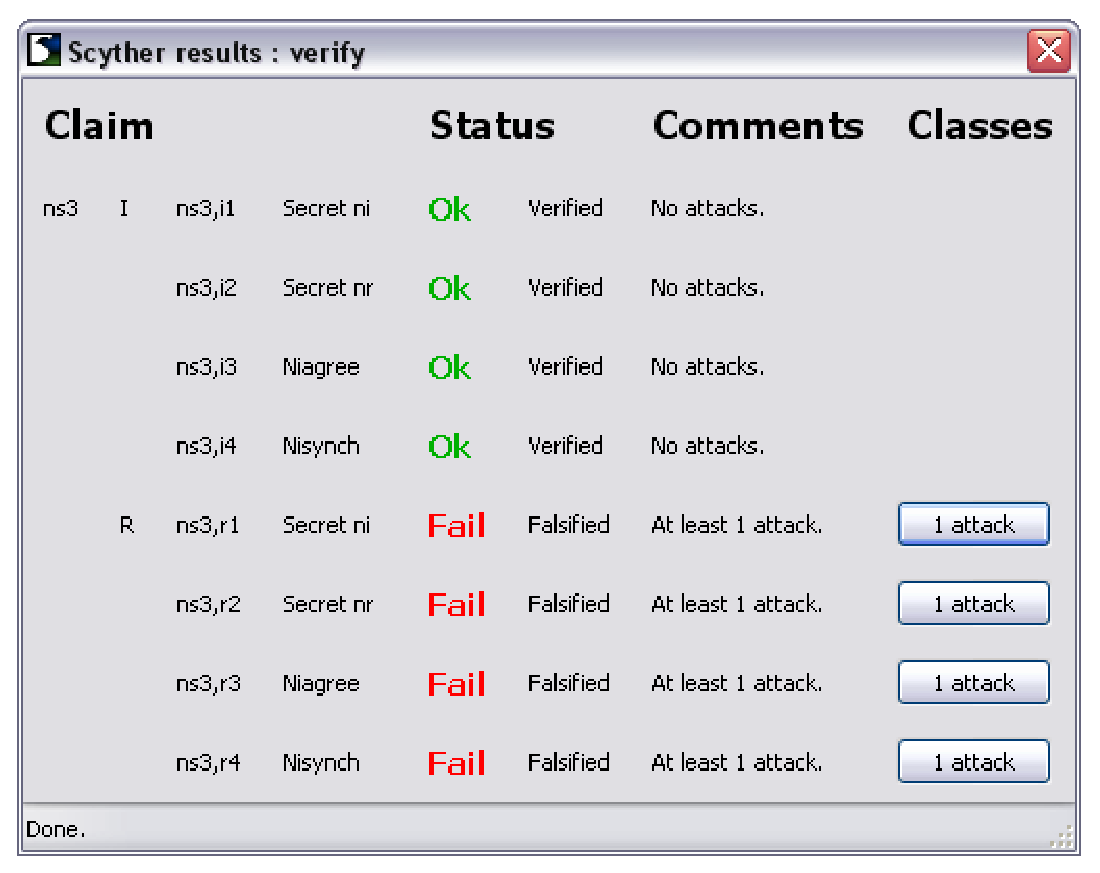
\includegraphics[scale=0.5]{resultwindow}
  \end{center}
  \label{resultwindow}
  \caption{Scyther result window}
\end{figure}

The result window shows a summary of the claims in the protocol, and the
verification results. Here one can find whether the protocol is correct,
or false. In the next section there will be a full explanation of the
possible outcomes of the verification process. Most importantly, if a
protocol claim is incorrect, then there exists at least one
attack on the protocol. A button is shown next to the claim: press this
button to view the attacks on the claim, as in
Figure~\ref{attackwindow}.

\begin{figure}[!htb]
  \begin{center}
    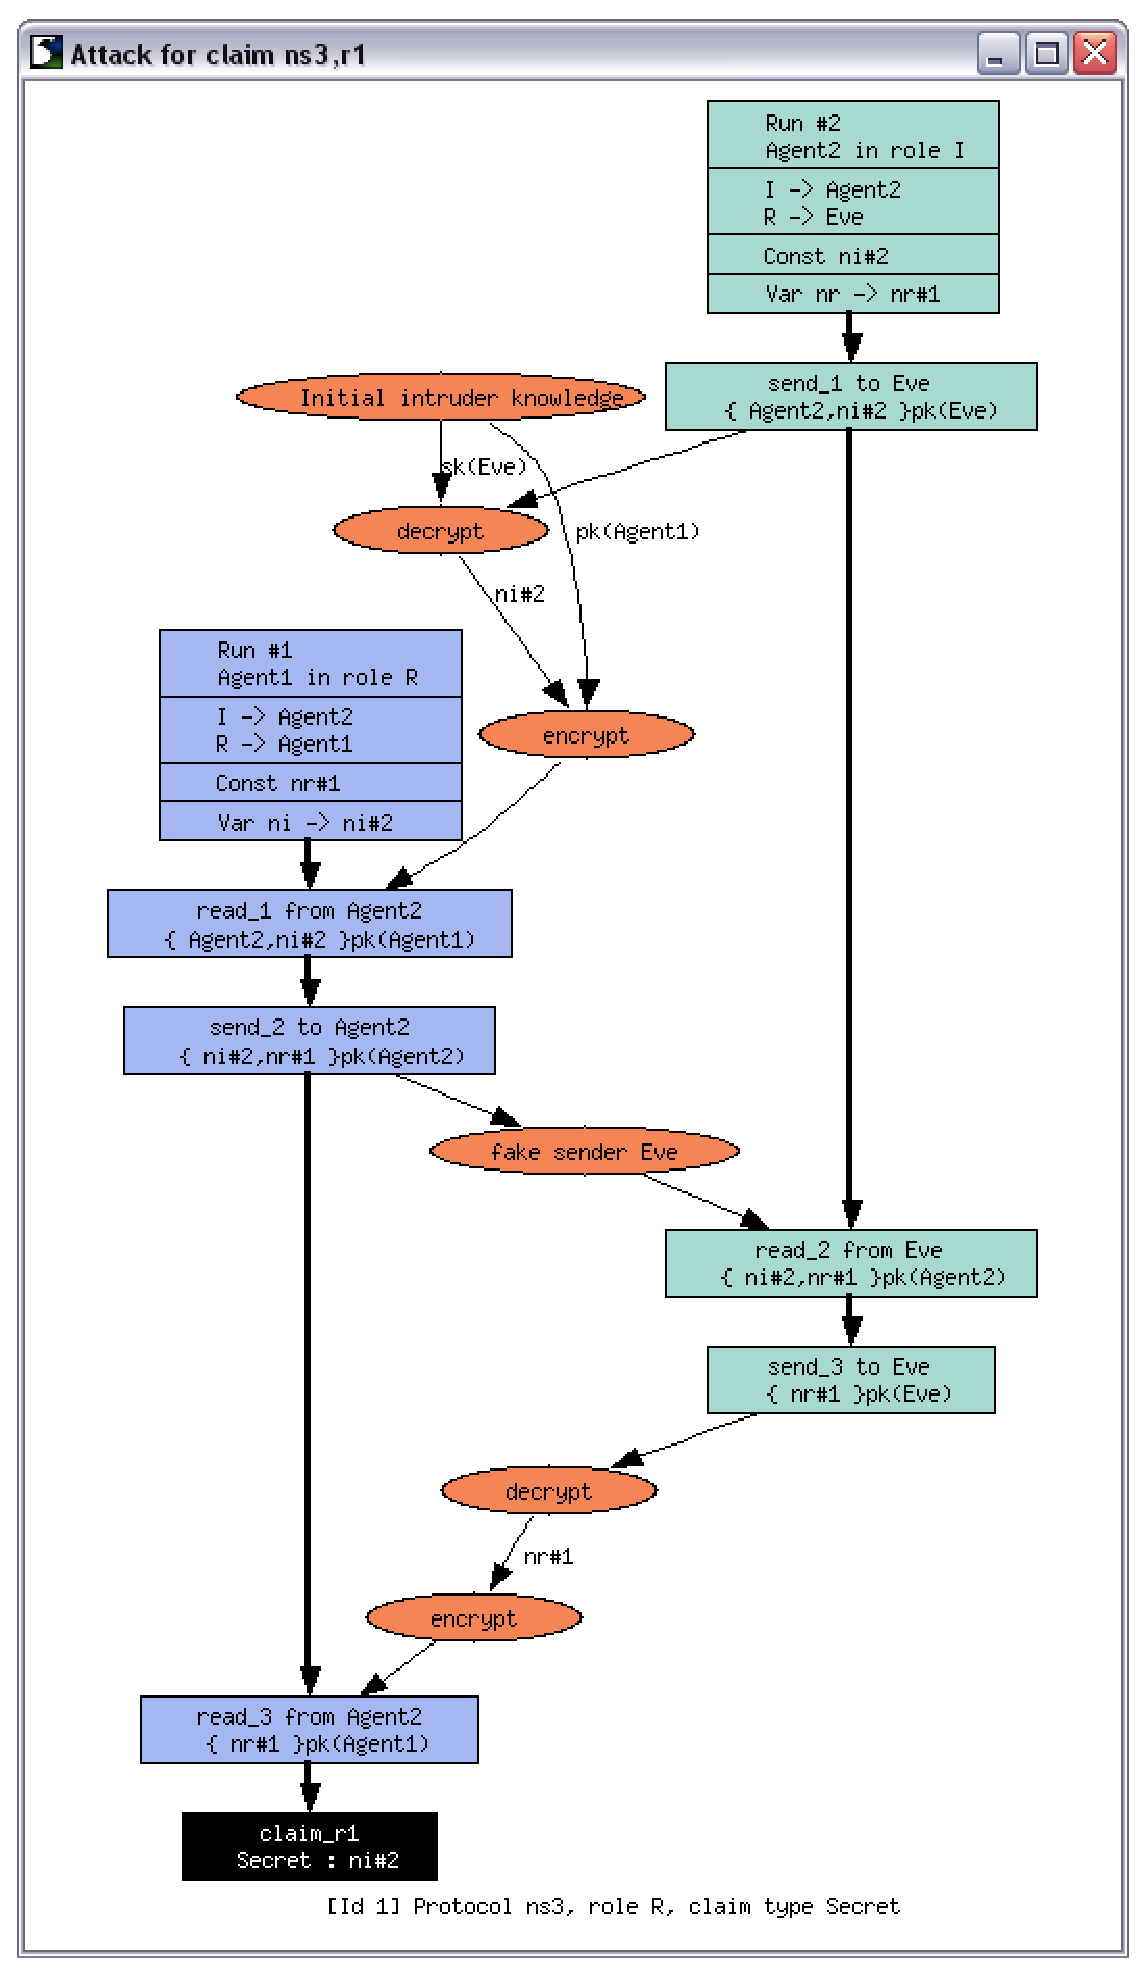
\includegraphics[height=0.90\textheight]{attackwindow}
  \end{center}
  \label{attackwindow}
  \caption{Scyther attack window}
\end{figure}


%----------------------------------------------------------------------------
\chapter{Input Language}
\label{sec:input}
%----------------------------------------------------------------------------

Scyther's input language is loosely based on a C/Java-like syntax.
The main purpose of the language is to describe protocols, which are defined by a set of
roles. Roles, in turn, are defined by a sequence of events, most of
which are events that denote the sending or receiving of terms. We describe
these elements in the following sections.

\index{comments}
Comments can start with \spd{//} or \spd{\#} (for single-line comments) or
be enclosed by \spd{/*} and \spd{*/} (for multi-line comments). Note that 
multi-line comments cannot be nested.

\index{whitespace}
Any whitespace between elements is ignored. It is
therefore possible to use whitespace (spaces, tabs, newlines) to
improve readability.

\index{identifier}
A basic identifier consists of a string of characters from
the set of alphanumeric characters as well as the symbols
\spd{\^{}} and \spd{-}.

\index{case-sensitive}
The language is case-sensitive, thus \spd{NS3} is not the same
identifier as \spd{ns3}.

%............................................................................
\section{A minimal input file}

The core elements in a Scyther input file are protocol definitions. A
minimal example is the following:
\begin{spdl}
protocol ExampleProtocol(I,R) {
  role I { };
  role R { };
};
\end{spdl}
In the above, we have defined a protocol called ``ExampleProtocol'' that
has two roles, ``I'' and ``R'' by listing them between brackets after
the protocol name. Note that we haven't defined the
behaviour of these roles
yet: such behaviours are defined within the curly brackets after the
corresponding \spd{role I} and \spd{role R} commands.


%............................................................................
\section{Terms}

At the most basic level, Scyther manipulates terms. 

\subsection{Atomic terms}

\index{atomic term}
An atomic term can be any identifier, which is usually a string of
alphanumeric characters.

Atomic terms can be combined into more complex terms by 
operators such as pairing and encryption.

\subsubsection{Constants}
\index{constant}
\index{global constant}

\subsubsection{Freshly generated values}
\index{freshly generated value}
\index{nonce}
\index{random value}

Many security protocols rely on generating random values. They can be
specified by declaring them inside a role definition using the
\spd{fresh} declaration. For example, to generate a random value
\scr{Na} of
type \spd{Nonce}, we specify:
\begin{spdl}
  role X(...) {
    fresh Na: Nonce;

    send_1(X,Y,Na);
  }
\end{spdl}

\subsubsection{Variables}
\index{variable}
\index{var}

Agents can use variables to store received terms. For example, to
receive a nonce into a variable with name \spd{Na}, we specify:
\begin{spdl}
  role Y(...) {
    var Na: Nonce;
    
    recv_1(X,Y,Na);
  }
\end{spdl}
Local declarations, for both freshly generated values as
well as variables such as \spd{Na}, are local to the role.
Thus, one can specify a \emph{freshly generated nonce} \spd{Na} in one
role and a variable \spd{Na} in another role without any conflicts.
Variables are rigid: after the first receive event in which they occur
has been executed, they are assigned a value. This value cannot be
changed afterwards.

Variables must occur first in receive events: it is not allowed to
use uninitialized variables in send events.

\subsection{Pairing}

\index{pairing}
\index{tupling}
Any two terms can combined into a term pair: we write \spd{(x,y)} for
the pair of terms \spd{x} and \spd{y}. It is also allowed to write
n-tuples as \spd{(x,y,z)}, which is interpreted by Scyther as \spd{((x,y),z)}.

\subsection{Symmetric keys}

\index{symmetric keys}
Any term can act as a key for symmetrical encryption.

The encryption of \spd{ni} with a term \spd{kir} is written as:
\begin{spdl}
{ ni }kir
\end{spdl}

Unless \spd{kir} is explicitly defined as being part of an asymmetric
key pair (explained below), this is interpreted as symmetric encryption.

\index{k(X,Y)@\spd{k(X,Y)}}
A symmetric-key infrastructure is predefined:
\spd{k(X,Y)} denotes the long-term symmetric key shared between $X$ and $Y$.

\subsection{Asymmetric keys}

\index{asymmetric keys}
\index{sk(X)@\spd{sk(X)}}
\index{pk(X)@\spd{pk(X)}}
A public-key infrastructure (PKI) is predefined:
\spd{sk(X)} denotes the long-term private key of $X$, and \spd{pk(X)}
denotes the corresponding public key.

\begin{example}

As an example, consider the following term. It represents the encryption
of some term \spd{ni} by the term \spd{pk(I)}. Under normal conventions,
this means that the nonce of the initiator (\spd{ni}) is encrypted with
the public key of the initiator.

\begin{spdl}
{ ni }pk(I)
\end{spdl}

This term can only be decrypted by an agent who knows the secret key
\spd{sk(I)}.

\end{example}

Section~\ref{adv:asymmetric} describes how to model more than one key
pair per agent.

\subsection{Hash functions}

\index{hash functions}
\index{hashfunction@\spd{hashfunction}}
Hash functions are essentially encryptions with a function, of which the inverse is not known by anybody.

They can be used by a global declaration of an identifier to be a
hashfunction, \eg:
\begin{spdl}
hashfunction H1;
\end{spdl}
As all agents and protocols should have access to such a function, the
declaration of hashfunction is usually global, \ie, defined outside of
any protocol definition.


\begin{example}
	Once declared, they can be used in protocol messages, \eg:
\begin{spdl}
H1(ni) 
\end{spdl}

\end{example}


\subsection{Predefined types}

\begin{description}

  \item [\spd{Agent }]

	  \spdindex{Agent}
  	Type used for agents.

  \item [\spd{Function }]

	  \spdindex{Function}
	A special type that defines a function term that can take a list
	of terms as parameter. By default, it behaves like a hash
	function: given the term \spd{h(x)} where \spd{h} is of type
	\spd{Function}, it is impossible to derive \spd{x}.

  \item [\spd{Nonce }]

	  \spdindex{Nonce}
  	A standard type that is often used and therefore defined inside
	the tool.

  \item [\spd{Ticket }]

	  \spdindex{Ticket}
	A variable of type \spd{Ticket} can be substituted by any term.

\end{description}

\subsection{Usertypes}

\spdindex{usertype}
It is possible to define a new type. This can be done
using the \spd{usertype} command:
\begin{spdl}
usertype MyAtomicMessage;

protocol X(I,R) {
   role I {
      var y: MyAtomicMessage;

      recv_1(I,R, y );
\end{spdl}
The effect of such a declaration is that variables of the new type can
only be instantiated with messages \spd{m} of that type, \ie, that have been
declared by the global declaration
\spd{const m: MyAtomicMessage}
or the freshly generated
\spd{fresh m: MyAtomicMessage} within a role.

In general, the tool can perform better if more is known about which messages might unify or not. By defining a usertype, the modeler can inform the tool that a variable can only be instantiated with terms of that type, and not with, \eg, terms of type Nonce.
Conceptually, one can always write \spd{Ticket} (which corresponds to all possible messages) for each variable type, but then one may find false attacks (in case the implementation in fact does check the type of a message) and the tool will be less likely to verify the property (for an unbounded number of runs).

\remark{CC}{Generic (local) declarations? Where is 'fresh' explained?}

\remark{CC}{TODO: reverse order: first protocol context, then roles,
then events. That way we can actually show what events can do.}

%............................................................................
\section{Events}
\index{events}

\subsection{Receive and send events}

\spdindex{send}
\index{event!send}
\index{event!recv}
\spdindex{send}
\spdindex{recv}
The \spd{recv} and \spd{send} events mark receiving and sending a
message, respectively. For example, we write:
\begin{spdl}
  role MyRole(...) {
    recv_Label1(OtherRole, MyRole, m1);
    send_Label2(MyRole, OtherRole, m2);
  }
\end{spdl}
to specify that role \spd{MyRole} first receives message \spd{m1} from
\spd{OtherRole} and then sends message \spd{m2} to \spd{OtherRole}. The
receive event is labeled with label \spd{Label1} and the send event is
labeled with \spd{Label2}.

Usually each \spd{send} event will have a corresponding \spd{recv}
event. We specify this correspondence by giving corresponding events the same
label.
\begin{spdl}
  role MyRole(...) {
    send_Label3(MyRole, OtherRole, m2);
  }
  role OtherRole(...) {
    recv_Label3(MyRole, OtherRole, m2);
  }
\end{spdl}


\subsubsection*{Bang prefix for labels}

For some protocols we may want to model sending or receiving to the
adversary directly, in which case we have no corresponding event.
If a \spd{send} or \spd{recv} event has no corresponding event, Scyther
will output a warning. To surpress this warning, the label can be
prefixed by a bang \spd{!}, \eg:
\index{20@{\tt "!}}
\begin{spdl}
send_!1(I,I, LeakToAdversary );
\end{spdl}


\subsection{Claim events and Security properties}
\index{event!claim}
\index{claim event}
\index{security properties}

\spdindex{claim}
Claim events are used in role specifications to model intended security properties. For
example, the following claim event models that \spd{Ni} is meant to be
secret.
\begin{spdl}
claim(I, Secret, Ni);
\end{spdl}

There are several predefined claim types.

\begin{description}

	

  \item[\spd{Secret }]

	  \spdindex{Secret}
  	This claim requires a parameter term. Secrecy of this term is
	claimed as defined in~\cite{opsembook}.

  \item[\spd{SKR }]

	  \spdindex{SKR}
	  The verification condition for this claim is equivalent to the \spd{Secret} claim. 

	  The purpose of this claim is to additionally mark the parameter term as a session-key.
	  The consequence is that using the \emph{session-key reveal}
	  adversary rule will now reveal the parameter term.

	  If the \emph{session-key reveal} rule is not enabled, this
	  claim is identical to the \spd{Secret} claim.

  \item[\spd{Alive }]

	  \spdindex{Alive}
	  Aliveness (of all roles) as defined in~\cite{lowe97hierarchy}.

  \item[\spd{Weakagree }]

	  \spdindex{Weakagree}
	  Weak agreement (of all roles) as defined in~\cite{lowe97hierarchy}.

  \item[\spd{Commit}, \spd{Running } ]

	  \spdindex{Commit}
	  \spdindex{Running}
	  \index{agreement on data}
	  \index{data agreement}
	  \index{non-injective agreement}
	  Non-injective agreement with a role on a set of data
	  items~\cite{lowe97hierarchy} can be defined by
	  inserting the appropriate signal claims.
	  In this context, \spd{Commit} marks the effective claim, whose
	  correctness requires the existence of a corresponding
	  \spd{Running} signal in the trace.

	  These claims are used to model agreement over data, which is
	  explained in Section~\ref{sec:agreement}.





  \item[\spd{Nisynch }]

	  \spdindex{Nisynch}
	  \index{synchronisaton}
	  \index{non-injective synchronisation}
  	Non-injective synchronisation as defined in~\cite{opsembook}.

  \item[\spd{Niagree }]

	  \spdindex{Niagree}
	  \index{agreement (on messages)}
	  \index{message agreement}
	  \index{non-injective agreement}
  	Non-injective agreement on messages as defined in~\cite{opsembook}.

  \item[\spd{Reachable }]

	  \spdindex{Reachable}
	When this claim is verified, Scyther will check whether this
	claim can be reached at all. It is true iff there exists a trace
	in which this claim occurs. This can be useful to check if there
	is no obvious error in the protocol specification, and is in
	fact inserted when the \scr{--check} mode of Scyther is used.

  \item[\spd{Empty }]
	  \spdindex{Empty}
  	This claim will not be verified, but simply ignored. It is only
	useful when Scyther is used as a back-end for other verification
	means. For more on this, see Section~\ref{sec:advanced}.

\end{description}


\subsection{Internal computation/pattern match events}
\index{internal computation events}
\index{pattern match events}

We extend the basic set of events from~\cite{opsembook} with two events that can be used to
model internal computations.

\subsubsection[Match event]{Match event\supported{v1.1 and Compromise-0.8}}
\index{match event}
\index{event!match}

The first new event is the \spd{match} event, that is used to specify
pattern matching, \ie,
\begin{spdl}
  match(pt,m)
\end{spdl}
In operational terms, if there exists a well-typed substitution $\sigma$
such that $\sigma pt = m$, then this event can be executed. Upon
execution, the substitution is applied to the remaining events of the
role.

This event can be used to model various constructions, such as equality
tests, delayed decryption, checking commitments. They can also be used
to model internal computations to simplify specifications, \eg:
\begin{spdl}
  var X: Nonce;
  var Y;

  recv(R,I, X);
  match(Y, hash(X,I,R) );
  send(I,R, Y,{ Y }sk(I) );
\end{spdl}
In the above example, we could have replaced \spd{Y} by
\spd{hash(X,I,R)} throughout the specification, but this version avoid
replication.

\subsubsection[Not match event]{Not match event\supported{v1.1 and Compromise-0.8}}
\index{not match event}
\index{event!not match}

The second new event is the \spd{not match} event, that is used to specify
pattern matching, \ie,
\begin{spdl}
  not match(pt,m)
\end{spdl}
The operational interpretation is the opposite of the previous event. If
there is no substitution $\sigma$ such that $\sigma pt = m$, then the
event can be executed.

This event can be used to model, \eg, inequality constraints. For
example, the execution model allows by default agents executing
sessions with themselves. In some cases, we want to exclude such
behaviour, because the protocol disallows it. For example,
\begin{spdl}
  role A {
    not match(A,B);
    send (A,B, m1);
  }
\end{spdl}
models a role whose instances only send messages to other agents.

As a more advanced usage, \spd{match} and \spd{not match} can be used
together in two roles with a common starting sequence of events to model
\emph{if ... then ... else} constructions. 
% LATER (advanced topics)
% We will return to this issue in Section~\ref{}

%............................................................................
\section{Role definitions}

\index{role definition}
Role definitions are sequences of events, \ie, declarations, send,
receive, or claim events.

\begin{spdl}
role Server {
  var x,y,z: Nonce;
  fresh n,m: Nonce;

  send_1(Server,Init, m,n );
  recv_2(Init,Server, x,y, { z }pk(Server) );
}
\end{spdl}

%............................................................................
\section{Protocol definitions}

\index{protocol definition}
A protocol definition takes as a parameter a sequence of roles, which
are then defined within its body.

\begin{spdl}
protocol MyProt(Init,Resp,Server)
{
  role Init {
    ...
  }
  role Resp {
    ...
  }
  role Server {
    ...
  }
}
\end{spdl}

\subsection*{Helper protocols}
\index{helper protocol|textbf}
\index{19@"@}

It is possible to prepend an ``@'' symbol before a protocol name. This
has no effect on the protocol model, nor on the outcome of the analysis.
The ``@'' is only used when rendering output graphs: the intent is to mark
the protocol as a 
``helper protocol''. Such protocols are often used to model additional adversary
capabilities, see Section~\ref{sec:advanced} for examples.
When rendering output graphs, Scyther collapses role instances of helper
protocols into single nodes. This can make the graphs more readable.

\subsection*{Symmetric-role protocols}
\index{symmetric-role protocol|textbf}

Some adversary-compromise rules, such as $\mathit{SKR}$ and
$\mathit{LKR}_\mathit{aftercorrect}$ depend on a partnering function. For
protocols that are entirely symmetric in their roles and key
computations (such as HMQV), this is not the appropriate partnering
function. To use the correct partnering function, the protocol needs to
be annotated as a \emph{symmetric-role} protocol. This instructs Scyther
to use the appropriate partnering function.

\begin{spdl}
symmetric-role protocol MyProt(Init,Resp)
{
  role Init {
    ...
  }
  role Resp {
    ...
  }
}
\end{spdl}


%............................................................................
\section{Global declarations}

\index{global declarations}
In many applications global constants are used. These include, for
example, string constants, labels, or protocol identifiers.

\spdindex{const}
They are modeled and used in the following way:
\begin{spdl}
usertype String;
const HelloWorld: String;

protocol hello(I,R)
{
  role I {
    send_1(I,R, HelloWorld);
  }
  role R {
    recv_1(I,R, HelloWorld);
  }
}
\end{spdl}


%............................................................................
\section{Miscellaneous}

\subsection[Macro]{Macro\supported{v1.1 and Compromise-0.8}}
\spdindex{macro}
\index{abbreviate}
\index{define macro}
It is possible to define \emph{macros}, \ie, abbreviations for
particular term. 
The syntax used to define these abbreviations is the following:
\begin{spdl}
  macro MyShortCut = LargeTerm;
\end{spdl}
For example, for a protocol that contains complex
messages or repeating elements, macros can be used to simplify the
protocol specification:
\begin{spdl}
hashfunction h;

protocol macro-example-one(I,R) {
   role I {
      fresh nI: Nonce;
      macro m1 = h(I,ni);

      send_1(I,R, { m1 }pk(R) );
      claim(I, Secret, m1);
   }
   role R {
      var X: Ticket;

      recv_1(I,R, { X }pk(R) );
   }
}
\end{spdl}
Note that macros have \emph{global scope}, and are handled at the 
\emph{syntactical} level. This also allows for global abbreviations of
protocol messages, \eg:
\begin{spdl}
hashfunction h;
macro m1 = { I,R, nI, h(nI,R) }pk(R);

protocol macro-example-two(I,R) {
   role I {
      fresh nI: Nonce;

      send_1(I,R, m1 );
   }
   role R {
      var nI: Nonce;

      recv_1(I,R, m1 );
   }
}
\end{spdl}
Note that in the above example, \spd{nI} is a freshly generated nonce in
the I role, and a variable in the R role. Because the macro definitions
are unfolded syntactically, the same macro can be used to refer to both
terms.

\subsection{Include}
It is possible to import other files in a protocol specification:

\spdindex{include}
\index{import file}
\index{input file}
\begin{spdl}
include "filename";
\end{spdl}

where {\em filename} denotes the name of the file that will be included
at this point. Using this command, it is possible to share, \eg, a set of common
definitions between files. Typically this will include definitions for
the key structures, and (untrusted) agent names. Nested use of this
command is possible.

\subsection[one-role-per-agent]{one-role-per-agent\supported{v1.1 and Compromise-0.8}}
\spdindex{one-role-per-agent}
\index{one role per agent}
\index{multiple roles per agent}
The operational semantics allow agents to perform any roles, and even
multiple different roles in parallel. This modeling choice corresponds
to the worst possible scenario, in which the adversary has the most
options to exploit. However, in many concrete settings, agents perform
only one role. For example, the set of servers may be disjoint from the
set of clients, or the set of RFID tags may be disjoint from the set of
readers. In such cases, we do not need to consider attacks that exploit
that an agent can perform multiple roles. This can be modeled by the
following statement:
\begin{spdl}
option "--one-role-per-agent"; // disallow agents in multiple roles
\end{spdl}
This causes Scyther to ignore attacks in which agents perform multiple
roles. Phrased differently, this corresponds to the situation in which
each role is performed by a dedicated set of agents.

%............................................................................
\section{Language BNF}

\index{BNF}
The full BNF grammar for the input language is given below. In the
strict language definition, there are no claim terms such as
\spd{Niagree} and \spd{Nisynch}, and neither are there any predefined
type classes such as \spd{Agent}. Instead, they are predefined constant
terms in the Scyther tool itself. 

\subsection{Input file}

An input file is simply a list of spdl constructions, which are global
declarations or protocol descriptions.

\begin{grammar}

<spdlcomplete>	::= <spdl> \{ ';' <spdl> \}

<spdl>		::=  <globaldeclaration>
		\alt <protocol>
		% Only needed for modelchecker
		%\alt `run' <roleref> `(' <termlist> `)' `;'

\end{grammar}

\subsection{Protocols}

A protocol is simply a container for a set of roles. Because
we use a role-based approach to describing roles, the protocol container
in fact only affects the
naming of the roles: a role ``I'' in a protocol ``ns3'' will internally be assigned the
name ``ns3.I''. This is used to make role names globally unique.

\begin{grammar}

<protocol>	::= `protocol' <id> `(' <termlist> `)' `{' <roles> `}' [ `;' ]

\end{grammar}

\subsection{Roles}

\begin{grammar}

<roles>		::= <role> [ <roles> ]
		\alt <declaration> [ <roles> ]

<role>		::= [ `singular' ] `role' <id> `{' <roledef> `}' [ `;' ]

<roledef>	::= <event> [ <roledef> ]
		\alt <declaration> [ <roledef> ]

\end{grammar}

\subsection{Events}

\begin{grammar}

<event>		::= `recv' <label> `(' <from> `,' <to> `,' <termlist> `)' `;'
		\alt `send' <label> `(' <from> `,' <to> `,' <termlist> `)' `;'
		\alt `claim' [ <label> ] `(' <from> `,' <claim> [ `,'
		<termlist> ] `)' `;'

% Only needed for modelchecker
% <roleref>	::= <id> `.' <id>

<label>		::= `_' <term>

<from>		::= <id>

<to>		::= <id>

<claim>     ::= <id>


\end{grammar}
\subsection{Declarations}
\begin{grammar}

<globaldeclaration>	::= <declaration>
		\alt `untrusted' <termlist> `;'
		\alt `usertype' <termlist> `;'

<declaration>	::= [ `secret' ] `const' <termlist> [ `:' <type> ] `;'
		\alt [ `secret' ] `fresh' <termlist> [ `:' <typelist> ] `;'
		\alt [ `secret' ] `var' <termlist> [ `:' <typelist> ] `;'
		\alt `secret' <termlist> [ <type> ] `;'
		\alt `inversekeys' `(' <term> `,' <term> `)' `;'
		\alt `compromised' <termlist> `;'

<type>		::= <id>

<typelist>	::= <type> \{ `,' <type> \}

\end{grammar}
\subsection{Terms}
\begin{grammar}

<term>          ::= <id>
		\alt `{' <termlist> `}' <key>
		\alt `(' <termlist> `)'
		\alt <id> `(' <termlist> `)'

<key>		::= <term>

<termlist>	::= <term> \{ `,' <term> \}


\end{grammar}


%----------------------------------------------------------------------------
\chapter{Modeling security protocols}
\label{sec:modeling}
%----------------------------------------------------------------------------

\begin{figure}[!htb]
	\centering
  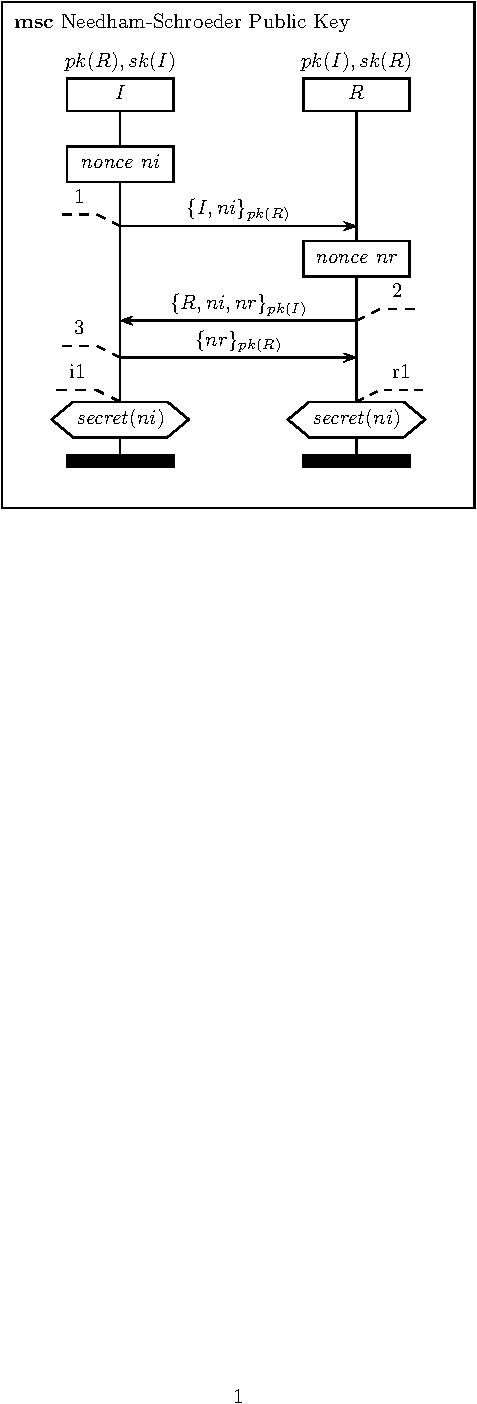
\includegraphics{msc-ns}
  \caption{A message sequence chart description}
  \label{msc:ns3}
\end{figure}

\section{Introduction}

The correct modeling of a security protocol for analysis in the Scyther
tool requires a basic understanding of the underlying 
symbolic model. This model is explained in detail in~\cite{opsembook}.

Roughly speaking, the symbolic analysis focuses on the following
aspects:
\begin{itemize}

	\item Logical message components and their intended function within the
		protocol (public versus
		secret, freshly generated in each run or constant)
	\item Message structure (pairing, encryption, signing, hashing)
	\item Message flow (order, involved agents)

\end{itemize}
Many other elements are abstracted away. For example, bit strings are
abstracted into terms, bit strings that occur with negligble probability
are abstracted away, and more complext control flow constructs such as
loops are often unfolded for a (low) finite number of times.

%The initial step of modeling a protocol typically takes the most time of
%the verification process. Most protocols are not very well documented,
%and because we work here with abstracted protocols, it is very easy to
%make a wrong abstraction in the process and miss out on a crucial
%feature. Once the protocol is modeled, the issue of deciding which
%security properties need to be included is often also unclear. Secrecy
%of some terms is fairly straightforward, but informal notions of
%authentication are potential minefields, and should be carefully
%examined.
%
%Once this difficult phase is over, and we are left with a
%suitable abstracted protocol, the tools can be used to quickly find
%attacks on the protocol model. It is often easy to check whether an
%attack on the abstract protocol constitutes an attack on the real
%protocol.

%............................................................................
\section{Example: Needham-Schroeder Public Key}

As an example, we show how to model a simple protocol.

\index{Needham-Schroeder protocol}
\index{NS|see{Needham-Schroeder protocol}}
Figure~\ref{msc:ns3} depicts the Needham-Schroeder Public Key protocol.
For simplicity, we have only displayed the claim by each role
that the initiator nonce $\nI$ is secret.

We start off the protocol description by adding a multi-line
comment that describes the protocol and other interesting details.
Multi-line comments start with \spd{/*} and end with \spd{*/}.
\begin{spdl}[numbers=left]
/* 
 * Needham-Schroeder protocol
 */
\end{spdl}

The protocol uses the default public/private key infrastructure: an agent
\spd{A} has
a key pair \spd{(pk(A),sk(A))}. 

The protocol has two roles: the
intiator role \spd{I} and the responder role \spd{R}. We also add a
single line comment, starting with \spd{//}.
\begin{spdl}[numbers=left,firstnumber=5]
// The protocol description

protocol ns3(I,R)
{
\end{spdl}

Scyther works with a role-based description of the protocols. We first
model the initiator role. This role has two values that are local to the
role: the nonce that is created by \spd{I} and the nonce that is
received. We have to declare them both.
\begin{spdl}[numbers=left,firstnumber=9]
  role I
  {
    fresh ni: Nonce;
    var nr: Nonce;
\end{spdl}

We now model the communication behaviour of the protocol.
Needham-Schroeder has three messages, and the initiator role sends the
first and last of these. Note the labels (\eg, \spd{\_1}) at the end of
the \spd{send} and \spd{recv} keywords: these serve merely to retain the
information of the connected arrows in the message sequence chart.

\begin{spdl}[numbers=left,firstnumber=14]
    send_1(I,R, {I,ni}pk(R) );
    recv_2(R,I, {ni,nr}pk(I) );
    send_3(I,R, {nr}pk(R) );
\end{spdl}

\remark{CC}{This should be refactored, and moved to the next chapter.}

Finally, we add the security requirements of the protocol. Without such
claims, Scyther does not know\footnote{If you are unsure about the
claims, you can also use the \scr{--auto-claims} switch to automatically
generate these at run-time.} what needs to be checked.

Here we have chosen to check for secrecy of the generated and received
nonce, and will check for non-injective agreement and synchronisation.
\begin{spdl}[numbers=left,firstnumber=18]
    claim_i1(I,Secret,ni);
    claim_i2(I,Secret,nr);
    claim_i3(I,Niagree);
    claim_i4(I,Nisynch);
  }  
\end{spdl}
This completes the specification of the initiator role.

For this simple protocol, the responder role is very similar to the
initiator role\footnote{In general, the transformation is not that
simple, but for many protocols this will suffice.}. In fact, there are
only a few differences:
\begin{enumerate}

  \item The keywords \spd{var} and \spd{fresh} have swapped places:
  \spd{ni} was created by \spd{I} and a freshly generated value there, but for the role
  \spd{R} it is the received value and thus a variable.

  \item The keywords \spd{send} and \spd{recv} have swapped places.

  \item The claims should have unique labels, so they have changed, and
  the role executing the claim is now \spd{R} instead of \spd{I}.

\end{enumerate}

The complete role description for the responder looks like this:
\begin{spdl}[numbers=left,firstnumber=24]
  role R
  {
    var ni: Nonce;
    fresh nr: Nonce;

    recv_1(I,R, {I,ni}pk(R) );
    send_2(R,I, {ni,nr}pk(I) );
    recv_3(I,R, {nr}pk(R) );

    claim_r1(R,Secret,ni);
    claim_r2(R,Secret,nr);
    claim_r3(R,Niagree);
    claim_r4(R,Nisynch);
  }
}
\end{spdl}

The full protocol description file for the {\em Needham-Schroeder}
protocol is given in Appendix~\ref{app:ns3}.



%----------------------------------------------------------------------------
\chapter{Specifying security properties}
\label{sec:properties}
%----------------------------------------------------------------------------

%\remark{CC}{This should synch up explicitly with the book chapter, and say
%where we deviate.}

\section{Specifying secrecy}



\section{Specifying authentication properties}

\subsection{Aliveness}

\subsection{Non-injective synchronisation}

\subsection{Non-injective agreement}

\subsection{Agreement over data}
\label{sec:agreement}
\spdindex{Commit}
\spdindex{Running}
\index{agreement on data}
\index{data agreement}
\index{non-injective agreement}

	  In order to specify data agreement, \eg, that the role $I$ agrees with
	  the role $R$ on a set of terms, \eg, the nonces
	  $ni$ and $nr$, one inserts two claims:
	  \begin{enumerate}
		  \item At the end of the $I$ role, insert
			  \spd{claim(I,Commit,R,ni,nr);}
		  \item In the $R$, just before the last send (in case
			  of a protocol with multiple roles: the last
			  send that
			  causally precedes the claim in the $I$ role),
			  insert
			  \spd{claim(R,Running,I,ni,nr);}

	  \end{enumerate}
  For an example of the use of these claims, see the ``ns3.spdl'' input file in the Scyther
  distribution. For a formal definition of the signals,
  see~\cite{lowe97hierarchy}.

%----------------------------------------------------------------------------
\chapter{Using the Scyther tool GUI}
\label{sec:gui}
%----------------------------------------------------------------------------

\index{GUI}
The Scyther tool can be used in two main ways. First, through the
graphical user interface (GUI) and second, through the command-line
interface. For most users the first option is preferred.

In this section we detail the Scyther output when used through the GUI.

%............................................................................
\section{Results}

As shown before, verifying the Needham-Schroeder public key protocol yields the
following results as in Figure~\ref{resultwindowbig}.

\begin{figure}[!htb]
  \begin{center}
    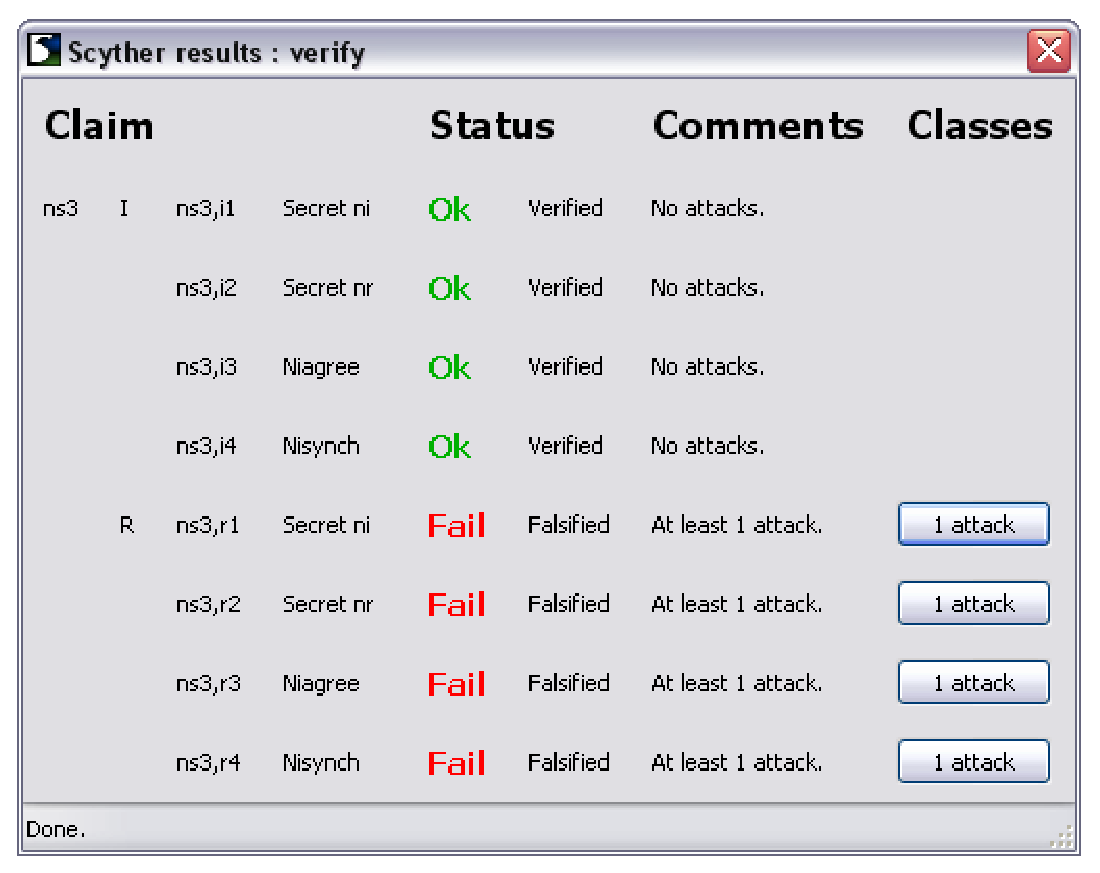
\includegraphics[width=\linewidth]{resultwindow}
  \end{center}
  \label{resultwindowbig}
  \caption{Scyther results for the Needham-Schroeder protocol}
\end{figure}

The interpretation is as follows: all the claims of the initiator role
\spd{ns3,I} are correct for an unbounded number of runs.

Unfortunately, all the claims of the responder role are false. Scyther
reports that it found at least one attack for each of those four claims.
We could choose to view these attacks: this will be shown in
Section~\ref{sec:graphical}.

In the result window, Scyther will output a single
line for each claim. The line is divided into several columns. The first
column shows the protocol in which the claim occurs, and the second
shows the role. In the third column a unique claim identifier is shown,
of the form \scr{p,l}, where \scr{p} is the protocol and \scr{l} is the
claim label.\footnote{This includes the protocol name, which is important when
doing multi-protocol analysis.}. The fourth column displays the claim
type and the claim parameter.

Under the header \scr{Status} we find two columns.
The fifth column gives the actual result of the verification process: it
will yield \scr{Fail} when the claim is false, and \scr{Ok} when the
claim is correct.
The sixth column refines the previous statement: in some cases, the
Scyther verification process is not complete (which will be explored in
more detail in the next section). If this column states \scr{Verified},
then the claim is provably true. If the column states \scr{Falsified},
then the claim is provably false. If the column is empty, then the
statement of fail/ok depends on the specific bounds setting.

The seventh column, \scr{Comments}, serves to explain the status of the results
further. In particular, the column contains a single sentences. We
describe the possible results below.

\begin{itemize}

	\item \scr{At least X attack(s)}

		\index{at least X attack(s)}
		Some attacks were found in the state space: however, due
		to the undecidability of the problem, or because of the
		branch and bround structure of the search, we cannot be
		sure that there are no other attack states.

		In the default setup, Scyther will stop the
		verification process after an attack is found.

	\item \scr{Exactly X attack(s)}

		\index{exactly X attack(s)}
		Within the statespace, there are exactly this many
		attacks, and no others.

	\item \scr{At least X pattern(s)}
	\item \scr{Exactly X pattern(s)}

		\index{exactly X pattern(s)}
		\index{at least X pattern(s)}
		These correspond exactly to the previous two, but occur
		in case of a `\spd{Reachable}' claim. Thus, the states
		that are found are not really attacks but classes of reachable
		states.

	\item \scr{No attacks within bounds}

		\index{no attacks within bounds}
		No attack was found within the bounded statespace, but there can
		possibly be an attack outside the bounded statespace.

	\item \scr{No attacks}

		\index{no attacks}
		\index{verification}
		No attack was found within the (bounded or unbounded) statespace, and a proof
		can be constructed that there is no attack even when the
		statespace is unbounded. Thus, the security property has
		been succesfully verified.

		Note that because of the nature of the algorithm, this
		result can even be obtained when the statespace is
		bounded.

\end{itemize}

%............................................................................
\section{Bounding the statespace}

During the verification process, the Scyther tool explores a proof tree
that covers all
possible protocol behaviours.  The default setting is to {\em bound} the
size of this tree in some
way, ensuring that the verification procedure terminates. However,
importantly, even if the size of this proof tree is bounded, unbounded
verification may still be achieved.

In most cases, the verification procedure will terminate and return
results before ever reaching the bound. However, if the verification procedure
reaches the bound, this is reported in the result window, \eg:

\begin{screen}
No attack within bounds
\end{screen}

This should be interpreted as: Scyther did not find any attacks, but
because it reached the bound, it did not explore the full tree, and it
is possible that there are still attacks on the protocol.

The default way of bounding the {\em maximum number of runs}, or protocol
instances. This can be changed in the \scr{Settings} tab of the main
window. If the maximum number of runs is, \eg, ~5, and Scyther reports
\scr{No attack within bounds}, this means that there exist no attacks
that involve 5 runs or less. However, there might exist attacks that
involve 6 runs or more.

For some protocols, increasing the maximum number of runs can lead to
complete results (i.e.~finding an attack or being sure that there is no
attack), but for other protocols the result will always be \scr{No
attack within bounds}.

Note that the verification time usually grows exponentially with respect
to the maximum number of runs.

%............................................................................
\section{Attack graphs}
\label{sec:graphical}

\index{attack graph}
\index{attack window}
In Figure~\ref{attackwindowbig} we show an attack window in more detail.

\begin{figure}[!htb]
  \begin{center}
    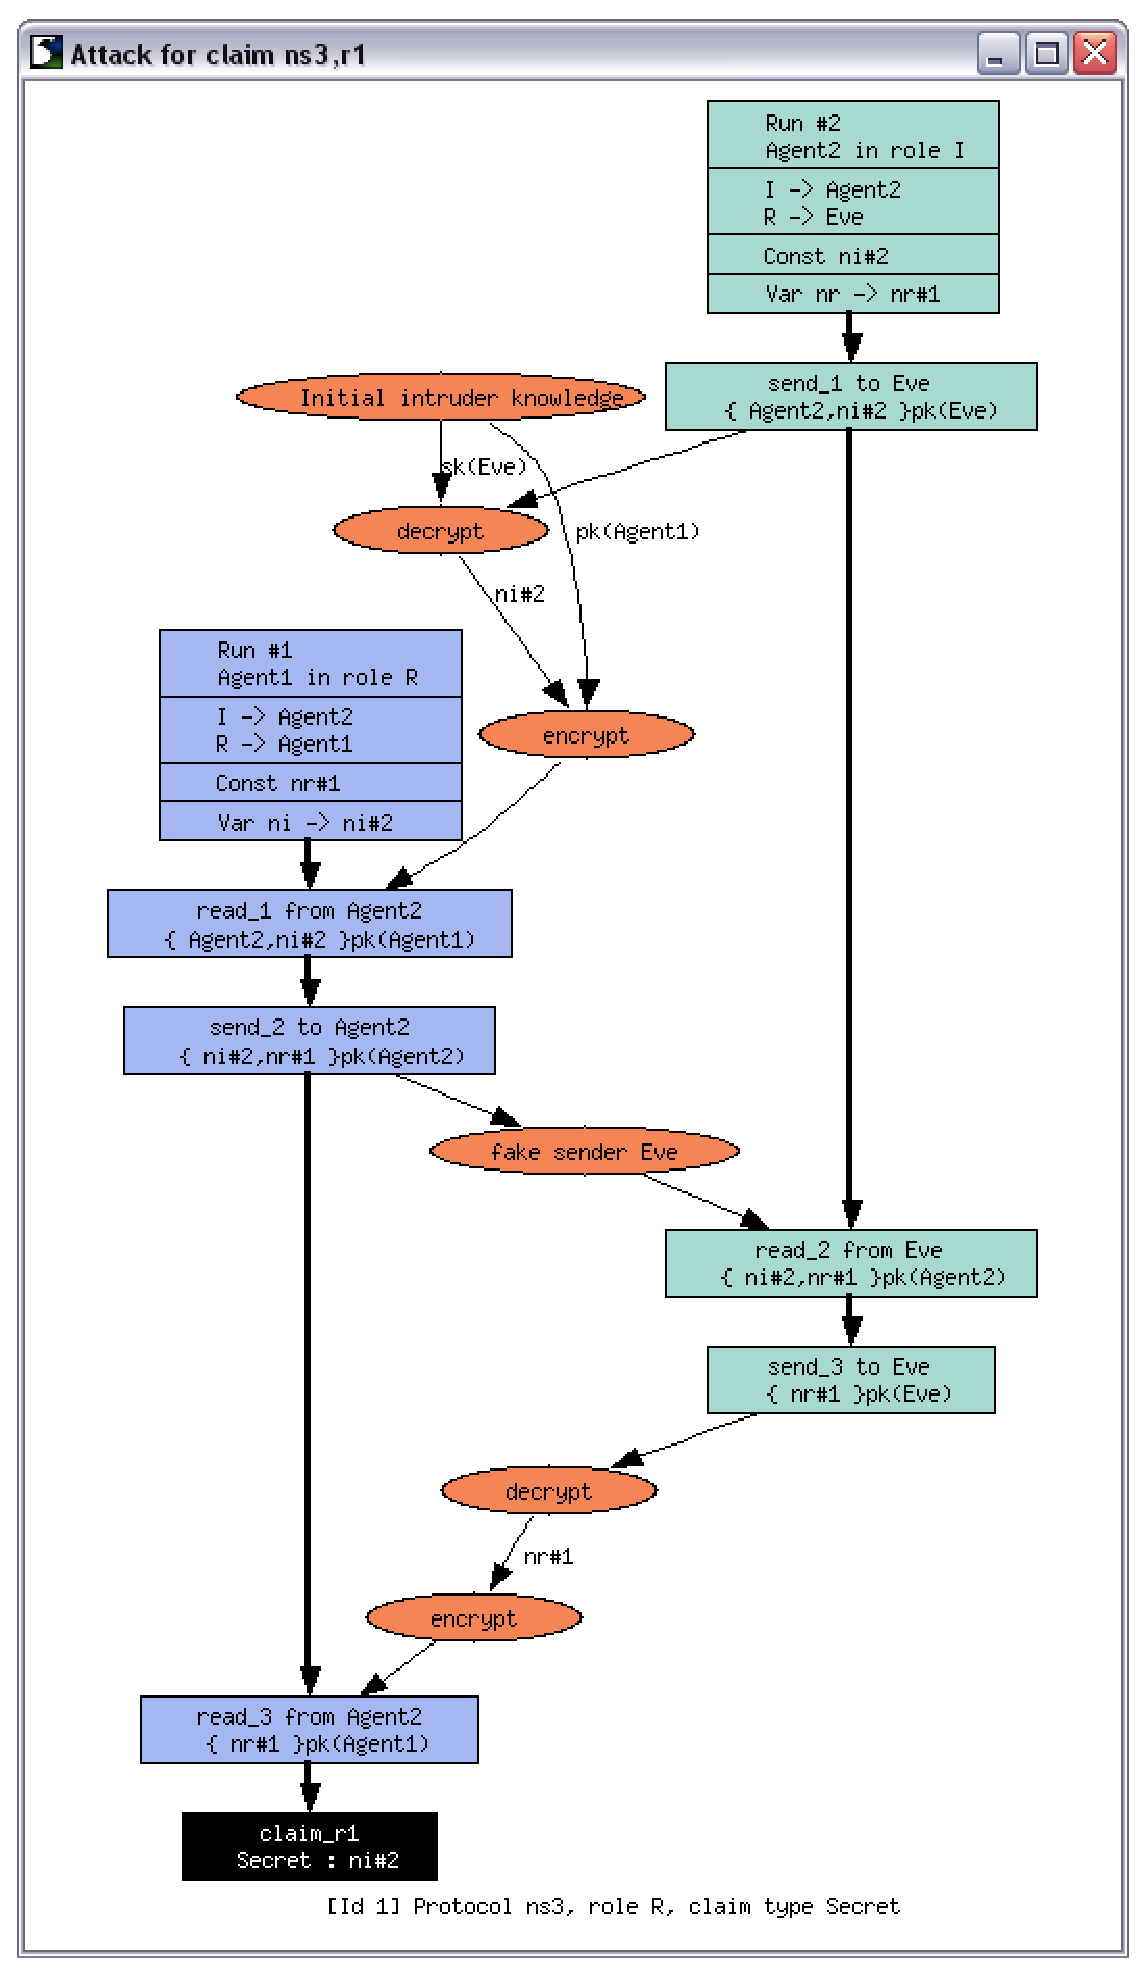
\includegraphics[scale=0.53]{attackwindow}
  \end{center}
  \label{attackwindowbig}
  \caption{Scyther attack window}
\end{figure}


The basic elements are arrows and several kinds of boxes. The arrows in
the graph represent ordering constraints (caused by the
prefix-closedness of events in the protocol roles, or by dependencies in
the intruder knowledge). The boxes represent creation of a run,
communication events of a run, and claim events.

\subsection{Runs}

\index{run}
Each vertical axis represents a run (an instance of a protocol role).
Thus, in this attack we see that there are two runs involved. Each run
starts with a diamond shaped box. This represents the creation of a run,
and is used to give information about the run.

For the run on the left-hand side in the attack we have this information:

\begin{ingraph}
Run #1
Agent2 in role I
I -> Agent2
R -> Agent1
\end{ingraph}

Each run is assigned a run identifier (here 1), which is an arbitrary
number that enables us to uniquely identify each run. This run executes
the \gra{R} role of the protocol. It is being executed by an agent
called \gra{Agent1}, who thinks he is talking to \gra{Agent2}. Note that
although run 2 is being executed by \gra{Agent2}, this agent does not
believe he is talking to \gra{Agent1}.

\begin{ingraph}
Run #2
Agent2 in role I
I -> Agent2
R -> Eve
\end{ingraph}

In the run on the right, we see
This run
represents an instance of the role \gra{I}.  From the second line we can
see which agent is executing the run, and who he thinks he is talking
to. In this example, the run is executed by an agent called
\gra{Agent2}, who thinks the responder role is being executed by the
untrusted agent \gra{Eve}.\footnote{Because this agent is talking to the
untrusted agent, of course all information is leaked, and no guarantees
can be given.}

Additionally, the run headers contain information on the freshly
generated values 
(\eg, run 1 generates \gra{nr\#1}) and information on the
instantiation of the local variables (\eg, run 1 instantiates its
variable \gra{ni} with the nonce \gra{ni\#2} or run 2.


\subsection{Communication events}

\index{communication event}
Send events denote the sending of a message. The first send 
occurs in this attack is the first send event of run 2.

\begin{ingraph}
send_1(Eve, { Agent#0, ni#2 }pk(Eve) )
\end{ingraph}

Every time a message is sent, it is effectively given to the intruder.
In this case, because the intruder knows the secret key \spd{sk(Eve)} of
the agent \gra{Eve}, he can decrypt the message and learns the value of
the nonce \gra{ni\#2}.

Receive events correspond to the successful reception of a message. The
first receive event that can
occur in this attack is the first receive event of run 0.

\begin{ingraph}
recv_1(Agent#0, { Agent#0, ni#2 }pk(Agent#1) )
\end{ingraph}

This tells us that the agent executing this run, \gra{Agent\#1}, reads a
message that is apparently coming from \gra{Agent\#1}. The message that
is received is \gra{\{ Agent\#0, ni\#2 \}pk(Agent\#1)} : the name of the
agent he thinks he is communicating with and the nonce \gra{ni\#2},
encrypted with his public key.

The incoming arrow does not indicate a direct sending of the message.
Rather, it denotes an ordering constraint: this message can only be
received
{\em after} something else has happened. In this case, we see that the
message can only be received after run 2 sends his initial message. The
reason for this is the nonce \gra{ni\#2}: the intruder cannot predict
this nonce, and thus has to wait until run 2 has generated it.

\index{construct}
In the graph the connecting arrow is red and has a label ``construct''
with it: this is caused by the fact that the message sent does not
correspond to the message that is received. We know the intruder can only
construct the message to be received after the sent message, and thus it
must be the case that he uses information from the sent message to
construct the message that is received. Other possibilities include a green
and a yellow arrow. A yellow arrow indicates that a message was sent,
and received in exactly the same form: however, the agents disagree about
who was sending a message to whom. It is therefore labeled with
``redirect'' because the intruder must have redirected the message. A
green arrow (not in the picture) indicating that a message is received
exactly the same as it was sent, representing a normal message
communication between two agents.

Note that a \spd{recv} event without an incoming arrow denotes that a term is
received that can be generated from the initial knowledge of the intruder.
There is no such event in the example, but this can occur often. For
example, if a role reads a plain message containing only an agent name,
the intruder can generate the term from his initial knowledge.

\subsection{Claims}

%----------------------------------------------------------------------------
\chapter{Using the Scyther command-line tools}
\label{sec:cli}
%----------------------------------------------------------------------------

\index{command-line tools}
\index{GUI!using Scyther without GUI}
All of the features offered by the Scyther GUI are also available
through command-line tools. Additionally, the command-line tools offer
some features that currently cannot be accessed through the GUI.

Depending on your platform, the Scyther directory contains one of the following executables:
\begin{itemize}
  \item \scr{Scyther/scyther-linux}
  \item \scr{Scyther/scyther-w32}
  \item \scr{Scyther/scyther-mac}
\end{itemize}
In the following, we assume that the linux version is used. If you have a different version, please replace \scr{scyther-linux} in the below by the executable for your platform.

To get a list of (some) of the command-line options, run the executable with the \scr{--help} switch, e.g.:
\begin{screen}
scyther-linux --help
\end{screen}
To analyze the Needham-Schroeder protocol and generate a .dot file (the input language for the Graphviz tool) for the attacks, use
\begin{screen}
scyther-linux --dot-output --output=ns3-attacks.dot ns3.spdl
\end{screen}
The resulting output file can then be rendered by graphviz, e.g.:
\begin{screen}
dot -Tpdf -O ns3-attacks.dot 
\end{screen}
This yields several PDF files \scr{ns3-attacks.dot[.N].pdf} that contain the attack graphs.

To get a more complete list of command-line options, run the executable with the \scr{--expert --help} switch, e.g.:
\begin{screen}
scyther-linux --expert --help
\end{screen}

%----------------------------------------------------------------------------
\chapter{Advanced topics}
\label{sec:advanced}
%----------------------------------------------------------------------------

\section{Modeling more than one asymmetric key pair}
\label{adv:asymmetric}

\index{multiple asymmetric key pairs per agent}
\index{asymmetric key!multiple pairs per agent}
Asymmetric keys are typically modeled as two functions: one function that maps
the agents to their public keys, and another function that maps agents to their
secret keys. 

By default, each agent $x$ has a public/private key pair
$(\spd{pk(x)},\spd{sk(x)})$.

To model other asymmetric keys, we first define the two functions, which are
for example named \spd{pk2} for the public key function, and \spd{sk2} for the secret
key function.
\begin{spdl}
const pk2: Function;
secret sk2: Function;
\end{spdl}

We also declare that these functions represent asymmetric key pairs:
\begin{spdl}
inversekeys (pk2,sk2);
\end{spdl}

If defined in this way, a term encrypted with \spd{pk2(x)} can only be
decrypted with \spd{sk2(x)} and vice versa.

\section{Approximating equational theories}

\index{equational theories}
\index{exponentiation|see{Diffie-Hellman exponentiation}}
\index{Diffie-Hellman exponentiation}
\index{bidirectional keys}
\index{syntactic equality}

The operational semantics underlying Scyther currently only consider
syntactic equality: two (ground) terms are equal if and only if they are
syntactically equivalent. However, there are several common
cryptographic constructions that are more naturally modeled by using certain
equalities. For example:
\begin{enumerate}
	\item $g^{ab} \; (\text{mod } N)$ and $g^{ba} \; (\text{mod }
		N)$, to model Diffie-Hellman exponentiation.
	\item $k(A,B)$ and $k(B,A)$, to model bidirectional long-term
		keys.
\end{enumerate}
Although Scyther does not provide direct support for such equational
theories, there exists a straightforward underapproximation.

The core idea is that instead of modeling the term equality, we
provide the adversary with the ability to learn all terms in an
equivalence class if he learns one of its elements.  For example, for
the equivalence class $\{ k(A,B), k(B,A) \}$ we can provide the
adversary with the ability to learn $k(B,A)$ from $k(A,B)$, and vice
versa. We can model this by introducing an appropriate helper protocol
(denoted by the prefix '@'):
\index{helper protocol}
\begin{spdl}
protocol @keysymmNaive(X) {
  role X {
    var Y: Agent;

    recv_!1(X,X,  k(X,Y)  );
    send_!2(X,X,  k(Y,X)  );
  }
}
\end{spdl}
Because the role can be instantiated for any agents $X$ and $Y$, this
covers all possible combinations of agents.

The above naive approximation can be significantly improved. One
obvious and practically relevant
omission is that the adversary usually learns encrypted messages, but
not the key. In such cases, we still would like to model
that \spd{\{ m \}k(A,B)} = \spd{\{ m \}k(B,A)}. Thus we adapt our helper
protocol:
\begin{spdl}
protocol @keysymmInefficient(X,Y) {
  role X {
    var Y: Agent;

    recv_!1(X,X,  k(X,Y)  );
    send_!2(X,X,  k(Y,X)  );
  }
  role Y {
    var X: Agent;
    var m: Ticket;

    recv_!1(Y,Y,  { m }k(X,Y)  );
    send_!2(Y,Y,  { m }k(Y,X)  );
  }
}
\end{spdl}
If the protocol contains further terms in which the symmetric keys
appear in other positions, such as in nested encryptions or hashes, we
would add further roles.
\remark{CC}{Maybe add pointer to more elaborate example in appendix?}

The above approximation is often inefficient in practice.
We can improve performance by making the helper protocol rules more
tight, \ie, by exploiting more type information about the protocol.
For example, if the protocol transmits two types of encrypted messages:
\begin{enumerate}
	\item \spd{ \{ I,nI,nR \}k(I,R) }, and
	\item \spd{ \{ nI \}k(I,R) },
\end{enumerate}
then we would modify the helper protocol in the following way:
\begin{spdl}
protocol @keysymm(X,Y,Z) {
  role X {
    var Y: Agent;

    recv_!1(X,X,  k(X,Y)  );
    send_!2(X,X,  k(Y,X)  );
  }
  role Y {
    var X,Z: Agent;
    var n1,n2: Nonce;

    recv_!1(Y,Y,  { Z,n1,n2 }k(X,Y)  );
    send_!2(Y,Y,  { Z,n1,n2 }k(Y,X)  );
  }
  role Z {
    var X,Y: Agent;
    var n1: Nonce;

    recv_!1(Z,Z,  { n1 }k(X,Y)  );
    send_!2(Z,Z,  { n1 }k(Y,X)  );
  }
}
\end{spdl}
In general, one would manually inspect the protocol and extract all
positions in which a term from an equivalence class occurs as a subterm.
For each of these positions, we model an appropriate role in the helper
protocols.

This is also used to model, for example, Diffie-Hellman
exponentiation. For exponentiation we introduce an abstract function
symbol, \eg, \spd{exp}, and a public constant \spd{g}. We then introduce
a helper protocol with roles to model that 
\spd{exp(exp(g,X),Y)} = 
\spd{exp(exp(g,Y),X)}.

In practice, this type of underapproximation has proven to be extremely
effective, to the point that all known attacks on real-world protocols
that can be modeled using the ``real'' equational theory, are found by
Scyther when using the underapproximation.

One caveat is that while this approximation works well for secrecy and
data-agreement, it can cause message-based agreement properties (such as
synchronisation) to fail, because their message equality checks are
syntactical. These checks are not affected by the introduction of helper
protocols.

%\section{Approximating undirected symmetric long-term keys}
% $k(A,B) = k(B,A)$
% Refer back to helper protocols

%\section{Approximating Diffie-Hellman}
% Refer back to helper protocols

% \section{Modeling internal checks}
% 
% \index{internal checks}
% \index{pattern matching}
% In most protocol models, the internal checks that a party performs
% when receiving a message are modeled by the pattern matching in the
% receive event. However, in some cases, this is not directly possible.
% For example, consider a protocol in which \spd{R} first receives
% an encrypted message \spd{\{knownString\}tempkey} that contains a
% specific constant encrypted with a fresh symmetric key. However,
% because $R$ does not have the key yet, he cannot decrypt the message,
% and simply stores the whole message in a variable \spd{T} of type Ticket. When
% \spd{R} later receives the key \spd{tempkey}, we would like to check that the message we
% received previously indeed is an encryption of the constant with the
% key, and abort if this is not the case. How can we model this?
% 
% What we would need in this case is an internal check that \spd{T} is
% equal to $\{knownString\}tempkey$. For example, we would like to have
% an
% event ``\spd{match(X,Y)}'' whose intuitive semantics are: if the pattern
% \spd{X} matches the ground term \spd{Y}, then proceed with those variable
% instantiations. If they cannot be unified, the event is blocked and will
% not be executed. Using such an event, we can trivially implement the
% above check.
% 
% Such a \spd{unify} event can be implemented in a role \spd{R} by the following
% specification:
% \begin{spdl}
%   fresh newmatchkey: Nonce;
%   send_!newlabel(R,R, { Y }newmatchkey);
%   recv_!newlabel(R,R, { X }newmatchkey);
% \end{spdl}
% Note that \spd{newmatchkey} and \spd{newlabel} can have any value, as
% long as they do not occur anywhere else in the protocol specification.
% If a protocol implements multiple \spd{unify} events, then each of these
% should use distinct term and label names.
% 
% This construction works because the fresh key is only used once. The
% adversary cannot learn the key; subsequently, there will be exactly one
% message that possibly matches the receive event. 
% 
% \index{delayed decryption}
% \index{committing to a term}
% \index{commit functionality}
% Using the above construction, protocols with delayed decryption, or that
% use hashes to implement ``committing to a term'' (commit functionality), can be modeled in a
% straightforward fashion.

\section{Modeling time-stamps and global counters}
\index{time-stamps|(}
\index{counter|see{global counter}}
\index{global counter|(}

Scyther's underlying protocol model currently does not provide support
for variables that are shared among the runs of an agent. Effectively, each run
starts with a ``clean slate'', independent of any runs that have been
executed previously. In other words, globally update state can not be
modeled directly.

In the following sections we provide some modeling approaches for
common problems. 

\subsection{Modeling global counters}

Globally incremented counters can be modeled using freshly generated
values. This ensures
that each run uses a different value. The model is coarse in the sense
that the recipient of such a
counter cannot check that it is the successor of the previous
value of the counter.

\index{global counter|)}

\subsection{Modeling time-stamps using nonces}

There are at least two ways to model time-stamps. 

The first model
is more appropriate for protocols where the probability that a given
time-stamp value is accepted by two runs is very low. This occurs when
time-stamps have great precision or when two runs occur only
sequentially, possibly with some delay time in between.
In this case, one can model time-stamps as freshly generated values,
\eg, nonces. To cater for the fact that the adversary typically knows
the time (and thus can also predict time-stamps), we prepend a
send event to the role that provides the adversary with the value of the
time-stamp that will be used. For example, we would
prepend the send with label \spd{!T1} for time-stamp \spd{T1} as in the
following example:
\begin{spdl}
usertype Timestamp;

protocol MyProtocol(Server,Client) {
  role Server{
    fresh T1: Timestamp;

    /* Time-stamps are unique per run */
    send_!T1(Server, Server, T1);

    ...
    /* Server uses time-stamp value */
    send_2(Server,Client, { Server, T1 }pk(Client) );
    ...
  }
}
\end{spdl}

\subsection{Modeling time-stamps using variables}

The second model is more appropriate when it is reasonable that two runs
may accept the same time-stamp value. This is common for coarse
time-stamps, or for roles that are typically executed with high
parallelism, such as server roles. In such cases, one can instead model
timestamps as values that are determined by the adversary.
In contrast to the previous solution, this is done by prepending a
receive event. For example:
\begin{spdl}
usertype Timestamp;

protocol MyProtocol(Server,Client) {
  role Server{
    var T1: Timestamp;

    /* Adversary chooses time-stamp value */
    recv_!T1(Server, Server, T1);

    ...
    /* Server uses time-stamp value */
    send_2(Server,Client, { Server, T1 }pk(Client) );
    ...
  }
}
\end{spdl}



\index{time-stamps|)}


\section{Multi-protocol attacks}
\label{sec:pma}
\index{multi-protocol attacks}
\index{cross-protocol attacks}
\index{chosen protocol attacks}

Scyther can be used to check for so-called \emph{multi-protocol attacks} (closely related concepts are \emph{cross-protocol attacks} and \emph{chosen protocol attacks}). These attacks depend on the interactions between different (sub)protocols: sometimes the adversary can use messages or message components from one protocol to attack another. For more information on this type of attack we refer to~\cite{Cr2006multiprotocol,kelsey97protocol}.

The easiest way to check for multi-protocol attacks in Scyther is to combine two protocol descriptions into a single file, i.e., create a new \scr{.spdl} file and paste into this file two other \scr{.spdl} files. The resulting file models an environment in which both protocols are running. Use Scyther to evaluate the claims in the combined file. 


%----------------------------------------------------------------------------
\chapter{Further reading}
\label{sec:further}
%----------------------------------------------------------------------------

% Note: this chapter should contain further reading that is purely tool
% related, such as protocol overviews, etc.


%==========================================================================
\bibliographystyle{plain}
\bibliography{biblio}
%==========================================================================

\appendix


%----------------------------------------------------------------------------
\chapter{Full specification for Needham-Schroeder public key}
\label{app:ns3}
%----------------------------------------------------------------------------

\begin{spdl}
/* 
 * Needham-Schroeder protocol
 */


// The protocol description

protocol ns3(I,R)
{
  role I
  {
    fresh ni: Nonce;
    var nr: Nonce;

    send_1(I,R, {I,ni}pk(R) );
    recv_2(R,I, {ni,nr}pk(I) );
    claim(I,Running,R,ni,nr);
    send_3(I,R, {nr}pk(R) );

    claim_i1(I,Secret,ni);
    claim_i2(I,Secret,nr);
    claim_i3(I,Alive);
    claim_i4(I,Weakagree);
    claim_i5(I,Commit,R,ni,nr);
    claim_i6(I,Niagree);
    claim_i7(I,Nisynch);
  }  
  
  role R
  {
    var ni: Nonce;
    fresh nr: Nonce;

   recv_1(I,R, {I,ni}pk(R) );
    claim(R,Running,I,ni,nr);
    send_2(R,I, {ni,nr}pk(I) );
    recv_3(I,R, {nr}pk(R) );

    claim_r1(R,Secret,ni);
    claim_r2(R,Secret,nr);
    claim_r3(R,Alive);
    claim_r4(R,Weakagree);
    claim_r5(R,Commit,I,ni,nr);
    claim_r6(R,Niagree);
    claim_r7(R,Nisynch);
  }
}
\end{spdl}

%==================================================
\chapter{Obsolete constructions}

\section{Read event}
\spdindex{read}%
Note that in some protocol description files one may find the \spd{read}
keyword: this is obsolete syntax and can safely be substituted by
\spd{recv}.



%==================================================

\printindex

\end{document}
